\documentclass[french]{book}
\usepackage[utf8x]{inputenc}
\usepackage[T1]{fontenc}
\usepackage{babel}
\usepackage{lmodern}
\usepackage[top=2cm,bottom=2cm,left=3cm,right=3cm]{geometry}
\usepackage{microtype}
\usepackage{mathtools, amssymb, amsthm}
\usepackage{mdframed}
\usepackage{hyperref}
\usepackage{graphicx}
\usepackage{xcolor}
\usepackage{mathrsfs}
\usepackage{wrapfig}
\usepackage{stmaryrd}

\newtheorem{prop}{Proposition}[section]
\newtheorem{theorem}{Théorème}
\newtheorem{definition}{Définition}[section]
\newtheorem*{remark}{Remarque}
\newtheorem*{lemma}{Lemme}
\newtheorem*{corollary}{Corollaire}
\newtheorem*{mth}{Méthode}
\newmdtheoremenv{thm}{Théorème}
\newtheorem{exo}{Exercice}
\newtheorem{exemple}{Exemple}


\newcommand{\lesss}{\rotatebox[origin=c]{90}{$\land$}}
\newcommand{\less}{\ \lesss\ }

\newcommand{\biggg}{\rotatebox[origin=c]{90}{$\lor$}}
\newcommand{\bg}{\ \biggg\ }

\title{\bsc{Théorie des représentations}}
\date{2023-2024}
\author{Yves \bsc{Aubry}, M-147A, yves.aubry@univ-tln.fr, Joachim \bsc{Asch}}

\begin{document}

\maketitle

\tableofcontents

\part{Représentations linéaires des groupes finis}

\chapter{Généralités sur les groupes}

\section{Rappels}


Soit $G$ un groupe. Soit $H$ un sous-groupe de $G$ (i. e. $H \neq 0$ et $\forall x, y \in H, x y ^{-1} \in H$).

Considérons la relation binaire suivante sur $G$ :

Pour $x, y \in G$, $x \equiv _{d} y \mod H$ ssi $x y ^{-1} \in H$. C'est une relation d'équivalence. Elle est dite de congruence à gauche modulo $H$.

\begin{proof}
  En effet, si $x \in G$, alors $x x ^{-1} = e \in H$, donc $x \mod _{g} = x \mod H$. La relation est donc réflexive.

  De plus, si $x, y \in G$ tels que $x \equiv _{g} y \mod H$, alors $x y ^{-1} \in H$. $H$ étant un sous-groupe de $G$, il est donc stable par passage au symétrique. D'où $(x y ^{-1} ) ^{-1}  \in H$, i. e. $y x ^{-1} \in H$, c'est-à-dire $y \equiv _{g} x \mod H$.

  Enfin, si $x, y,z \in G$ tels que $x \equiv _{g} y \mod H$ et $y \equiv _{g} z \mod H$, alors $x y ^{-1} \in H$ et $yz ^{-1} \in H$. Or, $H$ étant un sous-groupe de $G$, donc $H$ est stable pour la loi de composition interne. D'où $(x y ^{-1} )(y z ^{-1} ) \in H$. Par associativité, $x (y y ^{-1} ) z ^{-1}  \in H$, ie $x z ^{-1}  \in H$.

  Donc $x \equiv _{g} z \mod H $ et la relation est transitive.
\end{proof}

\

Soit $x \in G$. La classe d'équivalence de $x$ pour cette relation d'équivalence est

\begin{gather*}
  cl _{d}(x) = \{ y \in G \mid x y ^{-1} \in H \} \\
  = \{ y \in G \mid \exists h \in H, x y ^{-1} = h \} \\
  = \{ y \in G \mid \exists h \in H, y = hx \} \\
  = \{ hx, h \in H \} =: Hx
\end{gather*}

De même, on considère, sur $G$,  la relation de congruence à gauche modulo $H$  :

\begin{equation*}
  x \equiv _{g} y \mod H \text{ ssi } x ^{-1} y \in H.
\end{equation*}

On montre de même que c'est une relation d'équivalence. Si $x \in G$, alors $cl_g(x) := xH = \{ xh, h \in H \} $.

\begin{remark}
  Si $G$ est abélien, alors les classes à gauche et à droite modulo $H$ coincident.
\end{remark}

\begin{definition}
  Un sous-groupe $H$ d'un groupe $G$ est dit distingué dans $G$ (ou normal) si :

  \begin{gather*}
    \forall  x \in G, xH = Hx, \\
    \text{ i. e. } \forall x \in G, x H x ^{-1}  \subset H \\
    \text{ i. e. } \forall x \in G, x H x ^{-1} =H.
  \end{gather*}
\end{definition}

On note alors $H \triangleleft G$.

\begin{remark}
  Tout sous-groupe d'un groupe abélien est distingué.
\end{remark}

\begin{prop}
  Soit $G$ un groupe et $H$ un sous-groupe distingué de $G$.

  On note $G/H$ l'ensemble des classes à droite ou à gauche modulo $H$.

  Si $x, y \in G$ et si l'on note $\overline{a} $ la classe de $a$ modulo $H$, on peut munir le quotient $G/H$ d'une structure de groupe en posant

  \begin{gather*}
    \overline{x} \cdot \overline{y} = \overline{xy}.
  \end{gather*}
\end{prop}

\begin{proof}
  Cette loi est bien définie, i. e. elle ne dépend pas du choix des représentants des classes d'équivalence.
\end{proof}

\begin{remark}
  Cette loi de la surjection canonique $\pi:
    \begin{array}{lll}
    G & \longrightarrow & G/H \\
    x & \longmapsto \overline{x}
    \end{array}$ un morphisme de groupes.
\end{remark}

\begin{thm}[Lagrange]
  Soit $G$ un groupe fini et $H$ un sous-groupe de $G$.

  Alors l'ordre de $H$ divise l'ordre de $G$.
\end{thm}

\begin{remark}
  L'ordre d'un groupe est simplement son cardinal.
\end{remark}

\begin{remark}
  Si $g$ est un élément de $G$, alors l'ordre de $G$ est défini comme l'ordre du sous-groupe $\langle g \rangle $ engendré par $g$. S'il est fini, alors l'ordre de $g$ est le plus petit entier $n$ tel que $g ^{n} =e$.

  D'après le théorème de Lagrange, l'ordre d'un élément divise l'ordre du groupe.
\end{remark}

\begin{remark}
  Si $G$ est un groupe fini et $H$ un sous-groupe de $G$, alors les classes (à gauche) modulo $H$ ont toutes le même cardinal, à savoir celui de $H$. En effet, l'application, pour $x \in G : f_x:
    \begin{array}{lll}
    H & \longrightarrow & xH \\
    h & \longmapsto xh
    \end{array}$ est bijective.
\end{remark}

\section{Exemples de groupes}

\subsection{$ (\mathbb{Z}, +)$ }

Groupe abélien.

$n \mathbb{Z} = \{ nk, k \in \mathbb{Z} \} $ est un sous-groupe de $\mathbb{Z}$.

\begin{remark}
  Tout sous-groupe de $\mathbb{Z}$ est de la forme $n \mathbb{Z}$ pour un certain $n \mathbb{Z}$.
\end{remark}

\subsection{$\mathbb{Z}/{ n }\mathbb{Z}$}

C'est l'ensemble des classes d'équivalence pour la relation d'équivalence suivante :

\begin{gather*}
  x, y \in \mathbb{Z}, x \equiv y \mod n \mathbb{Z} \text{ ssi } x - y \in n\mathbb{Z}.
\end{gather*}

\begin{remark}
  $\overline{x} = \overline{y}  $ ssi $x R y$.
\end{remark}

On munit l'ensemble quotient $\mathbb{Z}/{ n }\mathbb{Z}$ d'une structure de groupe (et même d'anneau) en posant, pour $x, y \in \mathbb{Z}$ : $\overline{x}+ \overline{y} = \overline{x+y}   $ (et $\overline{x} \times \overline{y} = \overline{x \times y}   $).

\begin{remark}
  $\mathbb{Z}/{ 6 }\mathbb{Z}$ anneau non intègre, car $ \overline{2} \times \overline{3} = \overline{0}   $.
\end{remark}

\begin{remark}
  $\mathbb{Z}/{ n }\mathbb{Z}$ est un corps ssi $n$ est premier.
\end{remark}

\begin{prop}
  Tous les groupes $\mathbb{Z}/{ n }\mathbb{Z}$ sont cycliques. Les générateurs sont les $\overline{a} $ tels que $a$ et $n$ sont premiers entre eux, i. e. $(a,n) = 1$. De plus, tout groupe cyclique est isomorphe à $\mathbb{Z}/{ n }\mathbb{Z}$ avec $n = \lvert G \rvert$.

  Enfin, si $G$ est cyclique d'ordre $n$ alors pour tout diviseur $d$ de $n$, $G$ admet un sous-groupe d'ordre $d$, et celui-ci est unique, et celui-ci est cyclique.
\end{prop}

\begin{remark}
  $\mathbb{Z}/{ 2 }\mathbb{Z} \times \mathbb{Z}/{ 3 }\mathbb{Z} = \{ (\overline{a}, \tilde{a} ), \overline{a} \in \mathbb{Z}/{ 2 }\mathbb{Z}, \tilde{a} \in \mathbb{Z}/{ 3 }\mathbb{Z}  \} $.
\end{remark}

\begin{thm}[Théorème des restes chinois]
  Soient $n_1, \dots, n_r$ des entiers premiers entre eux deux à deux. Alors l'application

  \[
  \begin{array}{lll}
  \mathbb{Z}/{ \prod_{i=1}^{r} n_i  }\mathbb{Z} & \longrightarrow & \prod_{i=1}^{r } \mathbb{Z}/{ n_i }\mathbb{Z}  \\
  a + (\prod_{i=1}^{r} n_i ) \mathbb{Z} & \longmapsto (a+ n_1 \mathbb{Z}, \dots, a+ n_r \mathbb{Z})
  \end{array}
  \]

  est un isomorphisme d'anneaux et la réciproque est vraie.
\end{thm}

\marginpar{19-09-2023}

\section{Groupe diédral}

Soit $n \geq 3$ un entier. Le groupe diédral de degré $n$ est le groupe des isométries du plan laissant fixe le polygone régulier à $n$ côtés. On le note $D_n$ (ou $D _{2n}$).

$D_n$ est un groupe d'ordre $2n$ constitué de $n$ rotations et de $n$ symétries.

Considérons le polygone régulier dont les sommets sont, dans le plan complexe, les $n$ racines $n$-ièmes de l'unité :

\[
e^{\frac{2ik \pi}{n}}, k = 0, 1, \dots, n-1.
\]

\begin{figure}[h!]
  \centering
  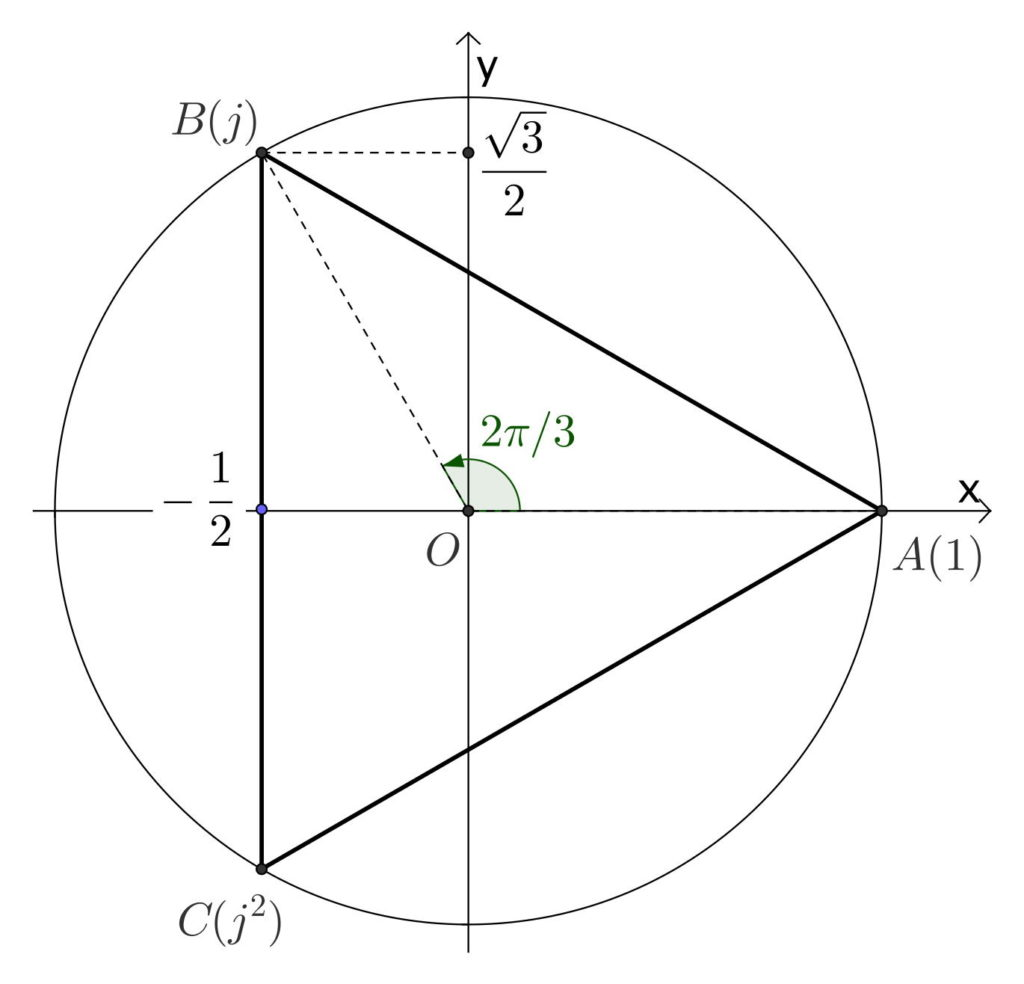
\includegraphics[scale=0.3]{figures/racines-3.jpg}
  \caption{Racines 3-ièmes de l'unité.}
  \label{}
\end{figure}

Soit $r = rot(0, \frac{2 \pi}{n})$ la rotation de centre $O$ et d'angle $\frac{2 \pi}{n}$ et soit $s$ la symétrie axiale d'axe la droite réelle $(x,x)$.

On a \[
r:\begin{array}{rcl}
\mathbb{C} & \longrightarrow & \mathbb{C} \\
z & \longmapsto e^{\frac{2 i \pi}{n}} z
\end{array}
\]

et

\[
s:
  \begin{array}{rcl}
  \mathbb{C} & \longrightarrow & \mathbb{C} \\
  z & \longmapsto \overline{z}
  \end{array}.
\]


On vérifie que l'on a $r ^{n} = 1 = id$, $s ^2 = 1 =id$ et $rs = r ^{-1} $.

\begin{proof}
  En effet, si $z \in \mathbb{C}$, alors

  \[
  r ^{-1} (z) = e^{- \frac{2 i \pi}{n}} z \text{ et } s r s(z) = s r (\overline{z} ) = s \left( e^{\frac{2 i \pi}{n}} \overline{z} \right) = e^{- \frac{2 i \pi}{n}} z = r ^{-1} (z),
  \]

  donc $s r s = r ^{-1} $.
\end{proof}

On peut donc définir le groupe diédral $D_n$ par ``générateurs et relations'' de la façon suivante :

\[
D_n = \langle r,s \rangle  \text{ avec } r ^{n} = s ^2 = 1 \text{ et } s r s = r ^{-1} .
\]

Le sous-groupe de $D_n$ engendré par $r$ est un sous-groupe d'ordre $n$ :

\[
\langle r \rangle = \{ r, r ^2, \dots, r ^{n-1}, id \} \simeq \mathbb{Z}/{ n }\mathbb{Z} .
\]

Il est d'indice 2 dans $D_n$, il est donc distingué dans $D_n$.

\subsection{Description du groupe $D_3$}

\begin{figure}[h!]
  \centering
  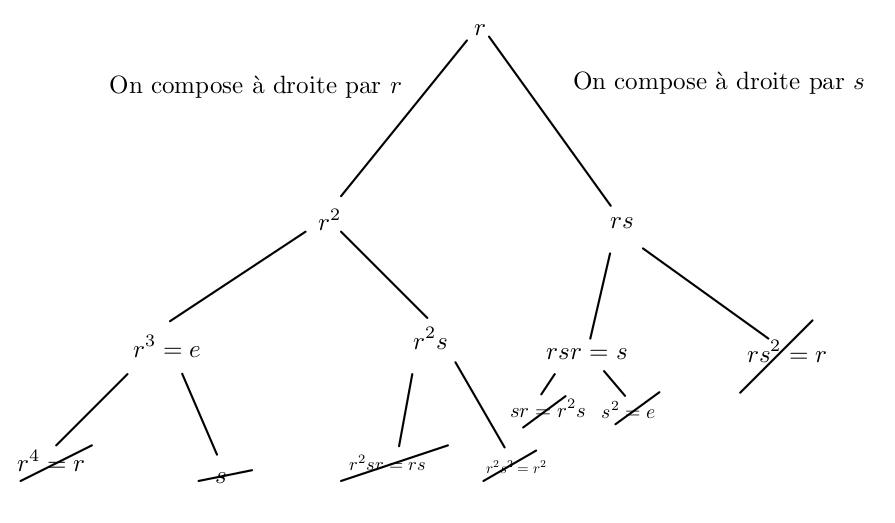
\includegraphics[scale=0.3]{figures/elts-d3.png}
  \caption{Description explicite des éléments de $D_3$.}
  \label{}
\end{figure}

On a donc

\[
D_3 = \{ e, r, r ^2, s, rs, r ^2 s \}
\]

\begin{remark}
  Il n'existe que deux groupes d'ordre 6 à isomorphisme près, à savoir le groupe cyclique (abélien) $\mathbb{Z}/{ 6 }\mathbb{Z}$ et le groupe symétrique (non abélien) $\mathfrak{S}_{3} $.
\end{remark}

Or $D_3$ n'est pas abélien, donc $D_3$ est isomorphe à $\mathfrak{S}_{3} $.

\begin{exo}
  Déterminer l'ordre des éléments de $D_3$ ainsi que ses sous-groupes.
\end{exo}

%\paragraph{Exemple du groupe quaternionien}

\begin{exemple}[Groupe quaternionien]
  Soit $\mathbb{H}$ le corps des quaternions d'Hamilton.

  \[
  \mathbb{H} = \{ a+ib+jc+kd \mid i ^2 = j ^2 = k ^2 = 1, ij = -ij = k, jk=-kj=i, ki=-ik=j \text{ et }  a, b, c, d \in \mathbb{R}\}.
  \]

  $\mathbb{H}$ est un corps non commutatif. On $\mathbb{R} \subset \mathbb{C} \subset \mathbb{H}$.

  Considérons le sous-ensemble suivant de $\mathbb{H}$ :

  \[
  \mathbb{H} _{8} = \{ 1, -1, i, -i, j, -j, k, -k \}.
  \]

  \begin{exo}
    Montrer que $\mathbb{H}_8$ muni de la multiplication est un groupe.
  \end{exo}

  C'est un groupe non abélien d'ordre 8.

  \begin{exo}
    Déterminer l'ordre des éléments de $\mathbb{H} _{8}$ ainsi que ses sous-groupes.
  \end{exo}
\end{exemple}



\paragraph{Rappel}


\begin{thm}[De classification des groupes abéliens finis]
  Tout groupe \textbf{abélien} fini est isomorphe à un produit de groupes cycliques de la forme

  \[
  \mathbb{Z}/{ d_1 }\mathbb{Z} \times \mathbb{Z}/{ d_2 }\mathbb{Z} \times \dots \times \mathbb{Z}/{ d_r }\mathbb{Z}, \text{ avec } d_1 \mid d_2 \mid \dots \mid d_r.
  \]

  Cette écriture est unique (à l'ordre près des facteurs).
\end{thm}

On en déduit qu'il existe trois groupes abéliens d'ordre 8 à isomorphisme près :

\[
\mathbb{Z}/{ 8 }\mathbb{Z}, \mathbb{Z}/{ 2 }\mathbb{Z} \times \mathbb{Z}/{ 4 }\mathbb{Z} \text{ et }  (\mathbb{Z}/{ 2 }\mathbb{Z}) ^3.
\]

Question : a-t-on $\mathbb{H}_8 \simeq D_4$ ?

\section{Les théorèmes de Sylow}

Si $H$ est un sous-groupe d'un groupe $G$, ses \textbf{conjugués} dans $G$ sont $g H g ^{-1} $, avec $g \in G$. En particulier, $H$ est distingué dans $G$ si et seulement si il est égal à tous ses conjugués.

\begin{definition}
  Si $G$ est un groupe fini d'ordre $p ^{\alpha} q$, avec $p$ premier, $\alpha \geq 1$ et $q$ premier avec $p$, alors tout sous-groupe de $G$ d'ordre $p3\alpha$ est appelé un $p$ sous-groupe de Sylow de $G$ (ou encore un $p$-Sylow de $G$).
\end{definition}

\begin{thm}[Premier théorème de Sylow]
  Soit $G$ un groupe d'ordre $p ^{\alpha} q$, $p$ premier, $\alpha \geq 1$, $(p, q)=1$. Pour tout $1 \leq \beta \leq \alpha$, il existe un sous-groupe de $G$ d'ordre $p ^{\beta}$.
\end{thm}

\begin{thm}[Deuxième théorème de Sylow]
  Le nombre $n_p$ de $p$-Sylow de $G$ vérifie :
  \[
  \begin{cases}
    n_p \equiv 1 \mod p \\
    n_p \mid q.
  \end{cases}
  \]
\end{thm}

\begin{thm}[Troisième théorème de Sylow]

  \

  \begin{enumerate}
    \item Le conjugué d'un $p$-Sylow est un $p$-Sylow.
    \item Tous les $p$-Sylow sont conjugués entre eux.
  \end{enumerate}
\end{thm}

\begin{exo}
  Montrer qu'il n'existe pas de groupes simples d'ordre 15.
\end{exo}

\begin{proof}
  Soit $G$ un groupe d'ordre $3 \times 5 = 15$. D'après le premier théorème de Sylow, $G$ admet au moins un 3-Sylow.

  Soit $n_3$ le nombre de 3-Sylow de G. Par le deuxième théorème de Sylow, on a

  \[
  n_3 \equiv 1 \mod 3 \text{ et } n_3 \mid 5.
  \]

  $G$ admet donc un unique 3-Sylow $H$.

  D'après le (1) du troisième théorème de Sylow, les conjugués de $H$ sont des 3-Sylow de $G$, donc sont égaux à $H$ puisque c'est le seul 3-Sylow de $G$. Donc $H$ est égal à tous ses conjugués et donc $H$ est distingué dans $G$. Puisque $\lvert H \rvert = 3$, $H \neq \{ e \} $ et $H \neq G$. Donc $G$ admet un sous-groupe distingué propre. Donc $G$ n'est pas simple.
\end{proof}

\subsection{Groupes agissant sur un ensemble ou action de groupes}

\begin{definition}[Action de groupe]
  Une action (à gauche) d'un groupe $G$ sur un ensemble $X$ est une application

  \[
    \begin{array}{lll}
    G \times X & \longrightarrow & X \\
    (g,x) & \longmapsto g \cdot x
    \end{array}
  \]

  telle que

  \begin{enumerate}
    \item $\forall x \in X, e \cdot x = x$ (où $e$ est l'élément neutre de $G$) ;
    \item $\forall g, g' \in G, \forall x \in X, g \cdot (g' \cdot x) = (gg')\cdot x$.
  \end{enumerate}
\end{definition}

On peut voir une action comme un morphisme de groupes de $G$ dans le groupe symétrique $\mathfrak{S}_{X} $ de permutations dans $X$ :

\begin{prop}
  Si un groupe $G$ agit sur un ensemble $X$ par

  \[
    \begin{array}{rcl}
    G \times X & \longrightarrow & X \\
    (g,x) & \longmapsto g \cdot x,
    \end{array}
  \]

  alors pour tout $g \in G$, l'application

  \[
  \pi_g:
    \begin{array}{rcl}
    X & \longrightarrow & X \\
    x & \longmapsto g \cdot x
    \end{array}
  \]

  est une permutation de $X$ et l'application

  \[
  \pi:
    \begin{array}{rcl}
    G & \longrightarrow & \mathfrak{S}_{X}  \\
    g & \longmapsto \pi_g
    \end{array}
  \]

  est un morphisme de groupes.

  Réciproquement, si $
    \begin{array}{rcl}
    G & \longrightarrow & \mathfrak{S}_{X}  \\
    g & \longmapsto p_g
    \end{array}$ est un morphisme de groupes, alors $(g,x) \mapsto g \cdot x :=p_g(x)$ est une action de $G$ sur $X$.
\end{prop}

\begin{proof}

  \

  %Vérifions que $\pi$ est bien un morphisme de groupes. Montrons tout d'abord que, si $g \in G$, alors l'application

  %\[
  %\pi:
  %  \begin{array}{rcl}
  %  X & \longrightarrow & X \\
  %  x & \longmapsto \pi_g(x) = g \cdot x
  %  \end{array}
  %\]

  %est une permutation de $X$.

  %On a

  %\[
  %\pi_e:
  %  \begin{array}{rcl}
  %  X & \longrightarrow & X \\
  %  x & \longmapsto x
  %  \end{array} = id_X.
  %\]

  %De plus, si $g, g' \in G$, alors $\pi _{gg'} = \pi_g \circ \pi _{g'}$.

  %Soit $x \in X$, on a $\pi _{gg'}(x) = (gg') \cdot x$ et

  %\begin{gather*}
  %  (\pi_g \circ \pi _{g'})(x)= \pi_g(\pi _{g'})(x)
  %\end{gather*}

  Supposons que $G$ agisse sur un ensemble $X$ par $
    \begin{array}{rcl}
    G \times X & \longrightarrow & X \\
    (g,x) & \longmapsto g \cdot x
    \end{array}$.

  Soit $g \in G$. Considérons l'application $\pi_g:
    \begin{array}{rcl}
    X & \longrightarrow & X \\
    x & \longmapsto g \cdot x
    \end{array}$.

  Montrons que $\pi_g$ est injective. Soient $x, y \in X$ tq $\pi_g(x) = \pi_g(y)$. D'où $g \cdot x = g \cdot y$. D'où $g ^{-1}  \cdot g \cdot x = g ^{-1}  \cdot g \cdot y$. D'où $(g ^{-1}  g ) \cdot x = (g ^{-1}  g ) \cdot y$. D'où $e \cdot x = e \cdot y$. Donc $\pi_g$ est injective. Montrons que $\pi_g$ est surjective. Soit $y \in X$. On a $y = \pi_g(g ^{-1}  y) = g \cdot g ^{-1}  \cdot y$. Donc $\pi_g$ est surjective. Donc $\pi_g$ est bijective.

  On peut donc considérer l'application $\pi:
    \begin{array}{rcl}
    G & \longrightarrow & \mathfrak{S}_{X}  \\
    g & \longmapsto \pi_g
    \end{array}$.

  Montrons que $\pi$ est un morphisme de groupes. Montrons que $\forall g, g' \in G, \pi _{g g'} = \pi_g \circ \pi _{g'}$.

  Soient $g, g' \in G$. Soit $x \in X$. $$\pi _{ gg'}(x) = (g g') \cdot x = g \cdot g' \cdot x = g \cdot (\pi _{ g'} (x)) = \pi_g (\pi _{ g'}(x)).$$

  Donc $\pi _{ gg'} = \pi_g \circ \pi _{ g'}$.

  \

  Réciproquement, si on se donne un morphisme de groupes d'un groupe $G$ dans un groupe de permutations $\mathfrak{S}_{X} $ :

  \[
  p:
    \begin{array}{rcl}
    G & \longrightarrow & \mathfrak{S}_{X}  \\
    g & \longmapsto p_g,
    \end{array}
  \]

  alors l'application

  \[
    \begin{array}{rcl}
    G \times X & \longrightarrow & X \\
    (g,x) & \longmapsto g \cdot := p_g(x)
    \end{array}
  \]

  est une action de groupes.

  En effet,

  \begin{enumerate}
    \item Soit $x \in X$, on a $e \cdot x = p_e(x) = id_X(x) = x$, car $p$ est un morphisme de groupes et l'image de l'élément neutre par un morphisme de groupes est l'élément neutre.
    \item Soient $g, g' \in G$ et soit $x \in X$ ; on a

    \begin{gather*}
      g \cdot (g' \cdot x) = g \cdot (p _{g'}(x)) = p_g(p _{g'}(x)) = (p_g \circ p _{g'})(x) = p _{gg'}(x) = (gg') \cdot x,
    \end{gather*}

    car $p$ est un morphisme de groupes.
  \end{enumerate}
\end{proof}

Cela établit deux bijections réciproques entre l'ensemble des actions de $G$ sur $X$ et celui des morphismes de $G$ dans $\mathfrak{S}_{X} $.

\begin{definition}
  Si un groupe $G$ agit sur un ensemble $X$, alors la relation sur $X$ définie par : pour $x, y \in X, x \sim y $ ssi $\exists g \in G, y = g  \cdot x$ est une relation d'équivalence. La classe d'équivalence de $X$ pour cette relation s'appelle \textbf{l'orbite} de $X$ :

  \[
  Orb(x):= \{ g \cdot x, g \in G \} .
  \]

  Ainsi, l'ensemble des orbites forme une \textbf{partition} de $X$.

  On dit que $g$ agit \textbf{transitivement} s'il n'y a qu'une seule orbite.

  Le \textbf{noyau} de l'action est le noyau du morphisme associé :

  \[
  \pi:
    \begin{array}{rcl}
    G & \longrightarrow & \mathfrak{S}_{X}  \\
    g & \longmapsto \left(\pi_g:
      \begin{array}{rcl}
      X & \longrightarrow & X \\
      x & \longmapsto g \cdot x
      \end{array}\right)
    \end{array}
  \]

  \[
  \operatorname{Ker}(\pi) = \{ g \in G \mid \forall x \in X, g \cdot x = x \}.
  \]

  On dit que l'action est \textbf{fidèle} si son noyau est réduit à $\{ e \} $ (i. e. si le morphisme $\pi$ est injectif).

  Le \textbf{stabilisateur} (ou groupe d'isotropie) d'un élément $x \in X$ est l'ensemble :

  \[
  Stab(x) = \{ g \in G \mid g \cdot x = x \}.
  \]

  C'est un sous-groupe de $G$ (en exercice).
\end{definition}

\begin{prop}
  Pour $x$ fixé dans $X$, l'application

  \[
    \begin{array}{rcl}
    G & \longrightarrow & X \\
    g & \longmapsto g \cdot x
    \end{array}
  \]

  définit une bijection de l'ensemble $G / Stab(x)$ des classes à gauche modulo $Stab(x)$ sur l'orbite de $x$. Ainsi, le cardinal de l'orbite $Orb(x)$ est égal à l'indice du stabilisateur de $x$ :

  \[
  \sharp(Orb(x)) = [G:Stab(x)].
  \]
\end{prop}

\begin{thm}[Formule des classes]
  Soit $G$ un groupe fini agissant sur un ensemble fini $X$. Alors

  \[
  \sharp(X) = \sum_{\substack{x \text{ décrivant un système} \\ \text{des représentants des orbites} }}^{} [G:Stab(x)].
  \]
\end{thm}

\begin{proof}
  \[
  \sharp(X) = \sum_{i=1}^{m} \sharp(Orb(x_i)),
  \]

  où $\{ x_1, \dots, x_n \}$ est un système des représentants des orbites pour l'action de $G$ sur $X$.
\end{proof}

\paragraph{Exemple d'action de groupe}

 On fait agit un groupe $G$ sur lui-même par conjugaison

 \[
   \begin{array}{rcl}
   G \times G & \longrightarrow & G \\
   (g,x) & \longmapsto g \cdot x := g x g ^{-1} .
   \end{array}
 \]

C'est bien une action de groupes, car

\begin{enumerate}
  \item Soit $x \in G$, on a $e \cdot x = e x e ^{-1} =x$.
  \item Soient $g, g' \in G$ et $x \in G$. On a :

  \[
  g \cdot (g' \cdot x) = g \cdot (g x g ^{-1} )=g(g'x (g')^{-1} ) g ^{-1} = (gg') x ((g')^{-1} g ^{-1} ) = (gg')x(gg') ^{-1} = (gg')\cdot x.
  \]
\end{enumerate}

\emph{Cette action est-elle transitive, fidèle ? Quelle est l'orbite d'un élément ?}

\marginpar{20-09-2023}

Soit $x \in G$. L'orbite de $x$ est :

\[
Orb(x) = \{ g \cdot x, g \in G \} = \{ g x g ^{-1} , g \in G \} = \text{classe de conjugaison de } x \text{ dans } G.
\]

On a $Orb(e) = \{ e \} $. Si $G$ n'est pas réduit à $\{ e \} $, il y a plusieurs orbites : l'action n'est donc pas transitive (il y a autant d'orbites que de classes de conjugaison).

\emph{L'action est-elle fidèle ?}  Etudions le noyau du morphisme $\pi$ associé à cette action

\[
\pi:
  \begin{array}{rcl}
  G & \longrightarrow & \mathfrak{S}_{G}  \\
  g & \longmapsto \left( \pi_g:
    \begin{array}{rcl}
    G & \longrightarrow & G \\
    x & \longmapsto g x g ^{-1}
    \end{array}\right).
  \end{array}
\]

On a

\begin{gather*}
  \operatorname{Ker}(\pi) = \{  g \in G \mid \pi_g =id_G \} = \{ g \in G \mid \forall x \in G, \pi_g(x) = x \} \\
  = \{ g \in G \mid \forall x \in G, g x g ^{-1} =x \} =  \{ g \in G \mid \forall x \in G, gx = xg \} = Z(G).
\end{gather*}

L'action est fidèle si et seulement si le centre de $G$ est réduit à l'élément neutre.

Soit $x \in G$. \emph{Quel est le stabilisateur de $x$ ?}

\begin{gather*}
  Stab(x) = \{ g \in G \mid g \cdot x = x \} = \{ g \in G \mid g x g ^{-1} =x \} = \{ g \in G \mid gx=xg \} = \text{centralisateur de } x.
\end{gather*}

Etudions un exemple avec $G = \mathfrak{S}_{3} $. Les orbites de $\mathfrak{S}_{3} $ pour cette action sont les classes de conjugaison de $\mathfrak{S}_{3} $. Elles constituent une partition de $\mathfrak{S}_{3} $.

\begin{enumerate}
  \item $Orb(e) = \{ e \} $.
  \item $Orb(\tau_3) = \{ \sigma \tau_3 \sigma ^{-1} , \sigma \in \mathfrak{S}_{3}  \} = \{ \text{transpositions de } \mathfrak{S}_{3} \} = \{ \tau_1, \tau_2, \tau_3 \} $.
  \item $Orb(\sigma_1) = \{ \sigma \sigma_1 \sigma ^{-1} , \sigma \in \mathfrak{S}_{3}  \} = \{ 3-\text{cycles de } \mathfrak{S}_{3}  \} = \{ \sigma_1, \sigma_2 \} $.
\end{enumerate}

La formule des classes s'écrit alors :

\[
\lvert \mathfrak{S}_{3} \rvert = \sum_{}^{} [\mathfrak{S}_{3}: Stab(x_i)],
\]

où $\{ x_1, x_2, x_3 \} $ est un système des représentants de l'orbite, avec $x_1 = e, x_2 = \tau_1, x_3 = \sigma_1$.

On a

\[
\lvert \mathfrak{S}_{3}  \rvert = \sum_{i=1}^{3} \sharp Orb(x_i)  =  \sharp Orb(x_1) +\sharp Orb(x_2) + \sharp Orb(x_3) =1+3+2 = 6.
\]

L'action est fidèle, car $Z(\mathfrak{S}_{3} ) = \{ e \} $. L'action n'est pas transitive, car il y a trois orbites, à savoir les trois classes de conjugaison.

\[
Stab(e) = \{ \sigma \in \mathfrak{S}_{3} \mid \sigma e = e \sigma \}= \mathfrak{S}_{3}.
\]

On a bien

\begin{gather*}
  [\mathfrak{S}_{3}: Stab(e) ] = \frac{\lvert \mathfrak{S}_{3}  \rvert}{\lvert Stab(e) \rvert} = \frac{3!}{3!}=1 = \sharp Orb(e).
\end{gather*}

On a $[\mathfrak{S}_{3}: Stab(\tau_3) ] = \sharp Orb(\tau_3) = 3$, donc $\lvert Stab(\tau_3) \rvert = 2$. D'où

\begin{gather*}
  Stab(\tau_3) = \{ \text{permutations de } \mathfrak{S}_{3} \text{ qui commutent avec } \tau_3 \} = \{ e, \tau_3 \}.
\end{gather*}

On a $[\mathfrak{S}_{3}: Stab(\sigma_1) ] = \sharp Orb(\sigma_1)=2$, donc $\lvert Stab(\sigma_1) \rvert = 3$. Puisque l'indice du stabilisateur est 2, on en déduit que $Stab(\sigma_1) \triangleleft \mathfrak{S}_{3} $. Or les seuls sous-groupes distingués de $\mathfrak{S}_{n} $ sont $\{ e \}, \mathfrak{S}_{n} \text{ et }  \mathfrak{A}_n  $. Donc

\begin{gather*}
  Stab(\sigma_1) = \mathfrak{A}_3 = \{ e, \sigma_1, \sigma_2 \}.
\end{gather*}

\chapter{Représentations linéaires des groupes finis}

Théorie introduite par Frobenius à la fin du XIX siècle.

\section{Premières définitions}

\begin{definition}
  Une représentation linéaire d'un groupe $G$ est la donnée d'un $\mathbb{C}$-espace vectoriel $V$ muni d'une action de groupes (à gauche) de $G$ agissant de manière linéaire :

  \[\begin{matrix}
    G \times V & \longrightarrow & V \\
    (g,x) & \longmapsto & g \cdot x
  \end{matrix}\]
  %  \begin{array}{rcl}
  %  G \times V & \longrightarrow & V \\
  %  (g,x) & \longmapsto g \cdot x
  %  \end{array}

  telle que

  \begin{enumerate}
    \item $\forall x \in V, e \cdot x = e$ ;
    \item $\forall g, g' \in G, \forall x \in V, g \cdot (g' \cdot x) = (gg')\cdot x$ ;
    \item $\forall g \in G, \forall x,x' \in V, \forall \lambda, \lambda' \in \mathbb{C}$, $g \cdot (\lambda x+\lambda'x') = \lambda g \cdot x + \lambda' g \cdot x$.
  \end{enumerate}
\end{definition}

Une représentation linéaire d'un groupe $G$ est donc la donnée d'un $\mathbb{C}$-espace vectoriel $V$ et d'un morphisme de groupes :

%\[
%\rho:
%  \begin{array}{rcl}
%  G & \longrightarrow & GL(V) \\
%  g & \longmapsto \left(\rho_g:
%    \begin{array}{rcl}
%    V & \longrightarrow & V \\
%    x & \longmapsto g \cdot x
%    \end{array}\right),
%  \end{array}
%\]


\[\begin{matrix}
\rho : & G & \longrightarrow & GL(V) \\
\ & g & \longmapsto & \left(\begin{matrix}
 V & \longrightarrow & V \\
 x & \longmapsto & g \cdot x
\end{matrix}\right)
\end{matrix}\]
où $GL(V)$ est le groupe des automorphismes du $\mathbb{C}$-espace vectoriel $V$.

On a bien $\forall g, g' \in G, \rho _{gg'} = \rho_g \circ \rho _{g'}$ et $\rho_e=id_V$ et $\rho _{g ^{-1} } = \rho_g ^{-1} $ comme vu précédemment.

De plus, $\forall  g \in G, $ la bijection $\rho_g$ est un endomorphisme de $V$, i. e. une application linéaire de $V$ dans $V$ et donc $\rho_g \in GL(V)$. En effet, si $x, x' \in V$ et $\lambda , \lambda' \in \mathbb{C}$, alors

\begin{gather*}
  \rho_g(\lambda x + \lambda' x') = g \cdot(\lambda x+ \lambda'x') \stackrel{(3)}{=} \lambda g \cdot x + \lambda' g \cdot x' = \lambda \rho_g(x) + \lambda'\rho_g(x').
\end{gather*}

\begin{definition}
  L'espace vectoriel $V$ est appelé \textbf{l'espace de la représentation}.

  La dimension de $V$ (en tant que $\mathbb{C}$-espace vectoriel) est appelé le \textbf{degré} ou la dimension de la représentation.

  Lorsque $\rho$ est injectif, la représentation est dite \textbf{fidèle} ; le groupe $G$ se représente alors de manière concrète comme un sous-groupe de $GL(V)$ ; lorsque $V$ est de dimension finie (ce que nous allons supposer dorénavant), le choix d'une base du $\mathbb{C}$-espace vectoriel $V$ fournit alors une représentation encore plus concrète comme groupe de matrice.
\end{definition}

\begin{remark}[Personnelle]
  Si \(\rho\) est une représentation fidèle, alors

  \[\operatorname{Ker}(\rho) = \{ g \in G \mid \forall x \in V, g \cdot x = x \} = \{ e \}. \]
\end{remark}

\begin{remark}
  Soient $G$ un groupe fini et $\rho : G \to GL(V)$ une représentation (linéaire) de $G$. Soit $g \in G$ un élément d'ordre $n$. On a alors

  \[
  (\rho_g)^n = \rho _{g ^{n}} = \rho_e = id_V.
  \]

  Donc l'endomorphisme $\rho_g$ est racine du polynôme $X^{n}-1$ qui n' a que des racines simples. Le polynôme minimal de $\rho_g$ divise donc le polynôme $X ^{n}-1$ et n'a donc aussi que des racines simples. Le polynôme minimal de $\rho_g$ est donc scindé sur $\mathbb{C}$ et à racines simples, on en déduit que l'endomorphisme de $\rho_g$ est \textbf{diagonalisable}.
\end{remark}

\paragraph{Exemples}

\begin{enumerate}
  \item La représentation triviale (ou représentation unité) :

  \[\begin{matrix}
  \rho : & G & \longrightarrow & GL(\mathbb{C}) \simeq \mathbb{C}^{*} \\
  \ & g & \longmapsto & \left( \rho_g : \begin{matrix}
   \mathbb{C} & \longrightarrow & \mathbb{C} \\
   x & \longmapsto & x
  \end{matrix}\right).
  \end{matrix}\]


    \item Les représentations de degré 1 : ce sont les morphismes de groupes

    \[
    \rho : G \longrightarrow \mathbb{C} ^{*}
    \]

    puisque si $dim V =1$, alors $GL(V) \simeq \mathbb{C}^{*}$, car les endomorphismes de $V$ sont des homothéties :

    %\[
    %f _{\lambda} : \mathbb{C} \longrightarrow \mathbb{C}, f _{\lambda}(x) = \lambda x
    %\]

    \[\begin{matrix}
    f _{\lambda } : & \mathbb{C} & \longrightarrow & \mathbb{C} \\
    \ & x & \longmapsto & \lambda x
    \end{matrix}\]

    et

    \[\begin{matrix}
      GL(V) & \longrightarrow & \mathbb{C} ^{*} \\
      f_{\lambda} & \longmapsto & \lambda
    \end{matrix}\]

    %\[
    %  \begin{array}{rcl}
    %  GL(V) & \longrightarrow & \mathbb{C} ^{*} \\
    %  f _{\lambda } & \longmapsto \lambda
    %  \end{array}
    %\]

    qui a une homothétie fait correspondre son rapport induit un isomorphisme. Si $G$ est \textbf{fini}, tout élément de $G$ est d'ordre fini (par le théorème de Lagrange) et donc, pour tout $g \in G$, $\rho_g$ est une racine de l'unité dans $\mathbb{C}$, et en particulier $\rho_g$ est un nombre complexe de module 1 :

    \[
    \lvert \rho_g \rvert = 1.
    \]

    \item Soient $\mathfrak{S}_n$ le groupe symétrique et $(e_1, \dots, e_n)$ la base canonique de $\mathbb{C} ^{n}$. On définit la représentation canonique de degré $n$ de $\mathfrak{S}_n$ en posant :

    \[\begin{matrix}
    \rho : & \mathfrak{S}_n & \longrightarrow & GL(\mathbb{C} ^{n}) \\
    \ & \sigma & \longmapsto & \left( \rho _{\sigma} : \begin{matrix}
    \mathbb{C} ^{n} & \longrightarrow & \mathbb{C}^{n} \\
    e_i & \longmapsto & \rho _{\sigma}(e_i) := e _{\sigma(i)}
    \end{matrix}\right).
    \end{matrix}\]

    %\[
    %\rho:
    %  \begin{array}{rcl}
    %  \mathfrak{S}_n & \longrightarrow & GL(\mathbb{C} ^{n}) \\
    %  \sigma & \longmapsto \left(\rho_\sigma:
    %    \begin{array}{rcl}
    %    \mathbb{C} ^{n} & \longrightarrow & \mathbb{C} ^{n} \\
    %    e_i & \longmapsto \rho _{\sigma}(e_i) := e _{\sigma(i)}
    %    \end{array}\right).
    %  \end{array}
    %\]

    \marginpar{26-09-2023}

    \item \emph{La représentation de permutations.} Soit \(\begin{matrix}
     G \times X & \longrightarrow & X \\
     (g,x) & \longmapsto & g \cdot x
   \end{matrix}\) une action d'un groupe sur un ensemble fini \(X\). Soit \(V\) un \(\mathbb{C}\)-espace vectoriel de dimension égale au cardinal de \(X\) (par exemple, on peut voir \(V\) comme le \(\mathbb{C}\)-espace vectoriel des fonctions définies sur \(X\) et à valeurs dans \(\mathbb{C}\) dont une base peut être donnée par les fonctions indicatrices \( \varepsilon_x : \begin{matrix}
     X & \longrightarrow & \mathbb{C} \\
     y & \longmapsto & \varepsilon_x(y) = \begin{cases}
      1 \text{ si } x=y \\
      0 \text{ sinon }
    \end{cases}
    \end{matrix}\) pour \(x\) décrivant \(X\)) muni d'une base indexée par les éléments de \(X\) : \(\{ \varepsilon_x, x \in X \} \). On peut écrire \(V = \bigoplus _{x \in X} \mathbb{C} \varepsilon_x\). On définit une représentation linéaire (complexe de dimension finie) :

    \[\begin{matrix}
    \rho : & G & \longrightarrow & GL(V) \\
    \ & g & \longmapsto &\left( \rho_g : \begin{matrix}
    V & \longrightarrow & V \\
    \varepsilon_x & \longmapsto & \rho_g(\varepsilon_x) := \varepsilon _{g \cdot x}
    \end{matrix} \right).
    \end{matrix}\]

    C'est la représentation de permutations associée à l'action de \(G\) sur \(X\) (c'est l'application qui envoie un vecteur de base sur un autre vecteur de base).

    \item \emph{La représentation régulière. } C'est l'exemple précédent avec \(X = G\) agissant sur lui-même (par translation à gauche) :

    \[\begin{matrix}
    \rho : & G & \longrightarrow & GL(V) \\
    \ & g & \longmapsto & \left( \rho_g : \begin{matrix}
    V & \longrightarrow & V \\
    \varepsilon_x & \longmapsto & \varepsilon _{gx}
    \end{matrix}\right).
    \end{matrix}\]

    Ici, il s'agit de la loi de composition interne de \(G\) et on a \(\operatorname{dim}(V) = \lvert G \rvert\).

\end{enumerate}

\begin{definition}
  Deux représentations linéaires \(\rho : G \to GL(V)\) et \(\rho' : G \to GL(V')\) d'un groupe \(G\) sont dites \textbf{isomorphes} ou équivalentes s'il existe un isomorphisme d'espaces vectoriels (ici application linéaire bijective) \(f: V \to V'\) tel que l'on ait : \[\forall g \in G, \rho'_g \circ f  = f \circ \rho_g.\]

  \begin{figure}[h!]
    \centering
    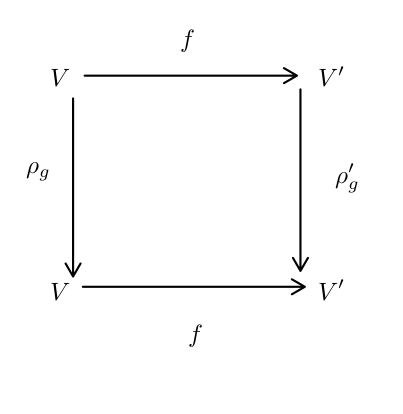
\includegraphics[scale=0.3]{figures/rep-iso2.png}
    \caption{Représentations linéaires isomorphes.}
    \label{}
  \end{figure}

  On peut exprimer cette condition par la commutativité du diagramme suivant :

  \begin{figure}[h!]
    \centering
    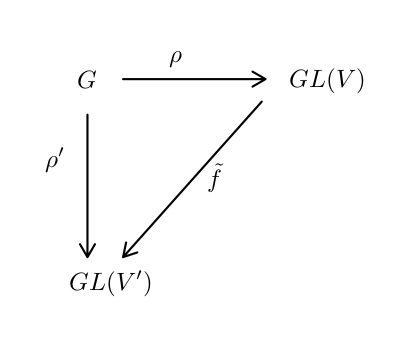
\includegraphics[scale=0.3]{figures/rep-iso.png}
    \caption{Diagramme commutatif de deux représentations isomorphes.}
    \label{}
  \end{figure}
\end{definition}

\begin{remark}
  Dire que le diagramme ci-dessus commute, c'est dire que

  \[\tilde{f} \circ \rho = \rho'.\]

  D'où, pour tout \(g \in G\), \(\rho'_g = \tilde{f} (\rho_g) = f \circ \rho_g \circ f ^{-1} \), i. e. \( \rho_g' \circ f = f \circ \rho_g\).
\end{remark}

\begin{remark}
  En termes de matrices, cela signifie  que les matrices associées à la première représentation sont semblable à leurs homologues dans la deuxième, via la même matrice de passage :

  \[\forall g \in G, \operatorname{Mat}(\rho_g') = \operatorname{Mat}(f) \times \operatorname{Mat}(\rho_g) \times \operatorname{Mat}(f) ^{-1}. \]
\end{remark}

\subsection{Sous-représentations}

\begin{definition}
  Si \(\rho : G \to GL(V)\) est une représentation linéaire d'un groupe \(G\) et si \(W\) est un sous-espace vectoriel de \(V\) stable par la représentation (i.e. stable par les automorphismes \(\rho_g\) pour \(g \in G\), i.e. \(\forall g \in G, \rho_g(W) \subset W\), i. e. \(\forall g \in G, \forall w \in W, \rho_g(w) \in W\)), alors cela nous permet de définir une \textbf{sous-représentation}

  \[\begin{matrix}
  \rho _{|W} : & G & \longrightarrow & GL(W) \\
  \ & g & \longmapsto & \left( \rho _{g _{|W}} : \begin{matrix}
  W & \longrightarrow & W \\
  w & \longmapsto & \rho_g(w)
  \end{matrix}\right).
  \end{matrix}\]
\end{definition}

\begin{definition}
  Une représentation \(\rho : G \to GL(V)\) est dite \textbf{irréductible} si les seuls sous-espaces stables de \(V\) sont \(\{0\} \text{ et } V\).
\end{definition}

\begin{remark}
  Les représentations de degré 1 sont bien évidemment des représentations irréductibles.
\end{remark}

\section{Théorème de Maschke}

On définit tout d'abord la notion de \textbf{somme directe} de représentations. On rappelle que si \(V\) est un espace vectoriel et si \(W, W'\) sont deux sous-espaces vectoriels de \(V\), alors on dit que \(V\) est \textbf{somme directe} de \(W\) et \(W'\) si tout \(x \in V\) peut s'écrire de façon unique sous la forme :

\[x = w+w', \text{ avec } w \in W, w' \in W'. \]

Il revient au même de dire que

\[W \cap W' = \{ 0 \} \text{ et } \operatorname{dim}(V) = \operatorname{dim}(W)+ \operatorname{dim}(W').\]

On écrit alors \(V = W \oplus W'\) et l'on dit que \(W'\) est un \textbf{supplémentaire} de \(W\) dans \(V\).

L'application \(p : \begin{matrix}
  V & \longrightarrow & V \\
  v = \underbrace{w}_{\in W} + \underbrace{w'}_{\in W'} & \longmapsto & w
\end{matrix}\) est alors appelé le \textbf{projecteur} de \(V\) sur \(W\) associé à la décomposition \(V = W \oplus W'\). On a \(\operatorname{Im}(p) = W\) et \(\operatorname{Ker}(p) = W'\) et \(p(x) = x\) si \(x \in W\).

Réciproquement, si \(p\) est une application linéaire de \(V\) sur lui-même vérifiant ces deux propriétés, on vérifie que \(V = W \oplus \operatorname{Ker}(p)\), avec \(\operatorname{Ker}(p) = \{ v \in V, p(v) = 0 \} \). On établit ainsi une \textbf{bijection} entre les projecteurs de \(V\) sur \(W\) et les \textbf{supplémentaires} de \(W\) dans \(V\).

\begin{definition}
  Soient \(\rho : G \longrightarrow GL(V) \text{ et } \rho' : G \longrightarrow GL(V')\) deux représentations d'un groupe \(G\). On définit la somme directe \(\rho \oplus \rho'\) comme étant la représentation d'espace vectoriel \(V \oplus V'\) définie par

  \[\begin{matrix}
  \rho \oplus \rho' : & G & \longrightarrow & GL(V \oplus V') \\
  \ & g & \longmapsto & \left( (\rho \oplus \rho')_g  : \begin{matrix}
  V \oplus V' & \longrightarrow & V \oplus V' \\
  v + v' & \longmapsto & \rho_g(v) + \rho_g'(v')
  \end{matrix}\right).
  \end{matrix}\]
\end{definition}

\begin{thm}[De Maschke]
  Toute représentation linéaire complexe de dimension finie d'un groupe fini est \textbf{somme directe de représentations irréductibles}.
\end{thm}

\begin{lemma}
  Tout sous-espace stable d'une représentation linéaire complexe de degré fini d'un groupe fini admet un sous-espace \textbf{supplémentaire \emph{stable}}.
\end{lemma}

\begin{remark}
  {\fontencoding{U}\fontfamily{futs}\selectfont\char 66\relax} Il existe un produit scalaire hermitien sur l'espace de la représentation qui est stable par l'action du groupe. En effet, si \(\langle \cdot, \cdot \rangle \) désigne un produit scalaire quelconque sur \(V\), le produit suivant est stable par \(\rho\) :

  \[\forall x, y \in V, \langle x, y \rangle_{\rho} := \frac{1}{\lvert G \rvert} \sum_{g \in G}^{} \langle \rho_g(x), \rho_g(y) \rangle. \]

  En effet, si \(h \in G\), alors on a:

  \begin{gather*}
    \langle \rho_h(x), \rho_h(y) \rangle _{\rho} = \frac{1}{\lvert G \rvert} \sum_{g \in G}^{} \langle \rho_g(\rho_h(x)), \rho_g (\rho_h(y)) \rangle  \\
    = \frac{1}{\lvert G \rvert} \sum_{g \in G}^{} \langle \rho _{gh}(x), \rho _{gh}(y) \rangle  = \langle x, y \rangle _{\rho},
  \end{gather*}

  car \(g \longmapsto gh\) est une bijection de \(G\) sur lui-même.
\end{remark}


\begin{proof}[Démonstration du lemme]
  Si \(W\) est un sous-espace vectoriel de \(V\) stable sous l'action de \(G\), alors le supplémentaire \textbf{orthogonal} de \(W\) est lui aussi stable sous l'action puisque : \(W \subset V\) stable sous l'action de \(G\) par \(\rho\), i. e. \( \forall g \in G, \rho_g(W) \subset W\). On a

  \[W ^{\perp} := \{  x \in V \mid \langle x, w \rangle _{\rho} = 0,  \forall w \in W \}.\]

  Montrons que \( W ^{\perp}\) est stable par \(\rho\). Soit \(g \in G\), soit \(x \in W ^{\perp}\), montrons que \(\rho_g(x) \in W ^{\perp}\). Soit \(w \in W\), montrons que \(\langle \rho_g(x), w \rangle _{\rho}=0\). On a

  \begin{gather*}
    \langle \rho_g(x), w \rangle_{\rho} = \langle \rho _{g ^{-1} }(\rho_g(x)), \rho _{g ^{-1} }(w) \rangle _{\rho} = \langle x, \rho _{g ^{-1} (w)} \rangle _{\rho} = 0,
  \end{gather*}

  car \(\rho _{g ^{-1} }(w) \in W\).
\end{proof}

\begin{proof}[Démonstration du théorème]
  Si \(\operatorname{dim}(V)=1\) ou si \(V\) est irréductible, c'est démontré.

  Si \(\operatorname{dim}(V) \geq 2\) et \(V\) est non irréductible, alors \(V\) possède une sous-représentation \(W\) distincte de \(\{ 0 \} \) et \(V\). Si \(\langle \cdot, \cdot \rangle _{\rho}\) est un produit scalaire hermitien sur \(V\) invariant sous l'action de \(G\), le supplémentaire orthogonal \(W ^{\perp}\) de \(W\) est lui aussi stable par \(G\). On a alors \(V = W \oplus W'\) et \(W\) et \(W'\) sont de dimensions inférieures à celle de \(V\).

  Par l'hypothèse de récurrence, on peut les décomposer en sommes directes de représentations irréductibles.
\end{proof}

\section{Caractère d'une représentation}

\begin{definition}
  On appelle \textbf{caractère} de la représentation \(\rho : G \longrightarrow GL(V)\) l'application

  \[\begin{matrix}
  \chi_{\rho} : & G & \longrightarrow & \mathbb{C} \\
  \ & g & \longmapsto & \chi_{\rho}(g) := \operatorname{Tr}(\rho_g).
  \end{matrix}\]

  où \(\operatorname{Tr}(\rho_g)\) désigne la \textbf{trace} de l'endomorphisme \(\rho_g\).

  Le degré du caractère \(\chi_\rho\) est défini comme le degré de la représentation \(\rho\).
\end{definition}

\begin{prop}[Propriétés du caractère d'une représentation]
  Soit \(\rho: G \longrightarrow GL(V)\) une représentation d'un groupe fini \(G\) de caractère \(\chi _{\rho}\).

  \begin{enumerate}
    \item \(\chi_{\rho}(e) = \operatorname{dim}(V) = \text{degré de } \rho = \text{degré de } \chi _{\rho}\).
    \item \(\forall g \in G, \chi _{\rho}(g ^{-1}) = \overline{\chi _{\rho}(g)}\) (conjugaison complexe).
    \item \(\forall g, h \in G\), \(\chi _{\rho}(g h g ^{-1} ) = \chi _{\rho}(h)\), i. e. \(\chi _{\rho}\) est une \textbf{fonction centrale} sur \(G\), i. e. \(\chi _{\rho}\) est \textbf{constante sur les classes de conjugaison}.
    \item \(\chi _{\rho\oplus \rho'} = \chi _{\rho}+ \chi _{\rho'}\), si \(\rho' : G \longrightarrow GL(V')\) est une représentation de \(G\).
    \item Si \(\rho, \rho'\) sont équivalentes, alors \(\chi _{\rho} = \chi _{\rho'}\).
  \end{enumerate}
\end{prop}

\marginpar{27-09-2023}

\begin{proof}

  \
  Soit \(\rho : G \longrightarrow GL(V)\) représentation linéaire d'un groupe fini \(G\) de caractère \(\chi _{\rho}\).
  \begin{enumerate}
    \item Par définition, \(\chi _{\rho}(e) = \operatorname{Tr}(\rho_e) \). Puisque \(\rho\) est un morphisme de groupes, l'image de l'élément neutre de \(G\) par \(\rho\) est donc l'élément neutre de \(GL(V)\), à savoir l'identité \(\operatorname{id}_V\) sur \(V\). D'où : \[\chi _{\rho}(e) = \operatorname{Tr}(\rho_e) = \operatorname{Tr}(id_V) = \operatorname{Tr}(I _{\operatorname{dim}(V)}). \]

    C'est la matrice identité à \(\operatorname{dim}(V)\) lignes et \(\operatorname{dim}(V)\) colonnes.

    \item Montrons que \(\forall g \in G, \chi _{\rho}(g ^{-1} ) = \overline{\chi _{\rho}(g)}\).

    Remarquons que si \(G\) est fini et si \(g \in G\), alors les valeurs propres de \(\rho_g\) (les racines du polynôme de cet endomorphisme) sont les racines de l'unité. En effet, si \(G\) est d'ordre \(n\), alors, par le théorème de Lagrange, on a \(g ^{n} = e\). D'où

    \[\rho_g ^{n} = \rho _{g ^{n}} = \rho_e = \operatorname{id}_V,\]

    donc le polynôme minimal de \(\rho_g\) divise \(X ^{n}-1\). Or les racines du polynôme minimal de \(\rho_g\) sont les valeurs propres de \(\rho_g\). Donc les valeurs propres de \(\rho_g\) sont les racines de l'unité.

    En particulier, les valeurs propres de \(\rho_g\) sont des nombres complexes de module 1. Donc, si \(\lambda \) est une valeur propre de \(\rho_g\), alors \(\lvert \lambda  \rvert = 1\) et donc \(\lambda  ^{-1} = \overline{\lambda }\). De plus, les valeurs propres de \(\rho _{g ^{-1}} = \rho _{g} ^{-1} \) (car \(\rho\) est un morphisme) sont les inverses de celles de \(\rho_g\).

    En effet, si \(f(x) = \lambda x\) avec \(x\) non nul et \(f \in GL(V)\), alors

    \[x =  f ^{-1} (f(x)) = f ^{-1} (\lambda x) = \lambda f ^{-1} (x),\]

    d'où \(f ^{-1} (x) = \lambda ^{-1} (x)\) et donc \(x\) est vecteur propre de \(f ^{-1} \) pour la valeur propre \(\lambda ^{-1} \).

    Enfin, puisque la trace d'un endomorphisme est la somme de ses valeurs propres (comptées avec leur multiplicités), on en déduit que

    \[\chi _{\rho}(g ^{-1}) = \overline{\chi _{\rho}(g)}. \]

    \item Soient \(g, h \in G\). On a

    \begin{gather*}
      \chi _{\rho}(g h g ^{-1}) \stackrel{\text{déf}}{=} \operatorname{Tr}(\rho _{ghg ^{-1}}) \stackrel{\text{morphisme}}{=} \operatorname{Tr}(\rho_g \circ \rho_h \circ \rho _{g ^{-1}}) \\
      = \operatorname{Tr}(\rho_g \circ \rho_h \circ \rho_g ^{-1}) \stackrel{\operatorname{Tr}(AB) = \operatorname{Tr}(BA)}{=} \operatorname{Tr}(\rho_g ^{-1} \circ \rho_g \circ \rho_h) = \operatorname{Tr}(\rho_h) = \chi _{\rho}(h).
    \end{gather*}

    Donc \(\chi _{\rho}\) est une fonction centrale sur \(G\), i. e. qu'elle prend les mêmes valeurs sur les éléments d'une même classe de conjugaison.

    \item Soient \(\rho : G \longrightarrow GL(V)\) et \(\rho' : G \longrightarrow GL(V')\) deux représentations de \(G\). La somme directe de \(\rho\) et \(\rho'\) est la représentation
     \[\begin{matrix}
      \rho \oplus \rho' : & G & \longrightarrow & GL(V \oplus V') \\
      \ & g & \longmapsto & \left( (\rho \oplus \rho')_g  : \begin{matrix}
      V \oplus V' & \longrightarrow & V \oplus V' \\
      v + v' & \longmapsto & \rho_g(v) + \rho_g'(v')
      \end{matrix}\right).
      \end{matrix}\]

      Si \((e_1, \dots, e_n)\) est une base de \(V\) et \((e_1', \dots, e_m')\) est une base de \(V'\), alors

      \[B = (e_1+0, \dots, e_n+0, 0 + e_1', \dots, 0 + e_m')\]

      est une base de \(V \oplus V'\).

      D'où

      \[\operatorname{Mat}_B((\rho \oplus \rho')_g) = \begin{pmatrix}
      \operatorname{Mat} _{(e_1, \dots, e_n)}(\rho_g) & 0 \\
      0 & \operatorname{Mat} _{(e_1', \dots, e_m')}(\rho_g')
      \end{pmatrix}, \]

      d'où

      \begin{gather*}
        \chi _{(\rho\oplus \rho')_g} = \operatorname{Tr}((\rho\oplus \rho')_g) = Tr(\operatorname{Mat}_B((\rho \oplus \rho')_g)) = \operatorname{Tr}(\operatorname{Mat} _{(e_1, \dots, e_n)}(\rho_g))+ \operatorname{Tr}(\operatorname{Mat} _{(e_1', \dots, e_m')}(\rho_g')) = \chi _{\rho}(g) + \chi _{\rho'}(g').
      \end{gather*}

      \item Soient \(\rho : G \longrightarrow GL(V)\) et \(\rho' : G \longrightarrow GL(V')\) deux représentations équivalentes de \(G\). Alors il existe une isomorphisme \(f : V \longrightarrow V'\) tel que

      \[\forall g \in G, \rho_g' = f \circ \rho_g \circ f ^{-1}.\]

      D'où, pour tout \(g \in G\), on a

      \[\chi _{\rho'}(g) = \operatorname{Tr}(\rho_g') = \operatorname{Tr}(f \circ \rho_g \circ f ^{-1}) = \operatorname{Tr}(\rho_g) = \chi _{\rho}(g).\]

      Donc \(\chi _{\rho} = \chi _{\rho'}\).
  \end{enumerate}
\end{proof}

\paragraph{Exemples de calculs de caractères}

\begin{enumerate}
  \item Si \(G\) opère sur un ensemble fini \(X\), considérons la représentation de permutations \(\rho\) associée, avec \(V = \bigoplus _{x \in X} \langle e_x \rangle = \bigoplus _{x \in X} \mathbb{C} e_x\).

  \[\begin{matrix}
  \rho : & G & \longrightarrow & GL(V) \\
  \ & g & \longmapsto &\left( \rho_g : \begin{matrix}
  V & \longrightarrow & V \\
  \varepsilon_x & \longmapsto & \rho_g(\varepsilon_x) := \varepsilon _{g \cdot x}
  \end{matrix} \right).
  \end{matrix}\]

  On a \(\chi _{\rho} : G \longrightarrow \mathbb{C}\) tel que \(\chi _{\rho}(g) = \operatorname{Tr}(\rho_g)\). Dans une base \((e_x) _{x \in X}\) de \(V\), pour \(g \in G\) fixé, la matrice de \(\rho_g\) est une matrice de permutations, i.e. a exactement un 1 par ligne et par colonne et tous les autres coefficients sont nuls.

  De plus, si \(\operatorname{Mat} _{(e_x)} (\rho_g) = (a _{ij}) _{i,j}\), alors le terme diagonal correspondant à \(\rho_g(e_x)\) sera égal à 1 si et seulement si \(g \cdot x = x\) si et seulement si \(x\) est un point fixe de \(g\). Sinon il vaudra 0. Donc

  \[\chi _{\rho}(g) = \operatorname{Tr}(\rho_g) = \sharp \{ x \in X \mid g \cdot x = x \}.\]

  \item \emph{Caractère de la représentation régulière (c'est le cas particulier de la représentation de permutations \(\rho\) avec \(G\) fini, \(X = G\), l'action étant la multiplication dans \(G\)).}

  On a alors, pour tout \(g \in G\) :

  \begin{gather}
    \chi _{\rho}(g) = \operatorname{Tr}(\rho_g) = \sharp \{ x \in G \mid g x=x \} = \begin{cases}
      \lvert G \rvert \text{ si } g=e \\
      0 \text{ si } g \neq e.
    \end{cases}
  \end{gather}
\end{enumerate}

\begin{definition}
  Un caractère d'un groupe \(G\) est dit \textbf{irréductible} si c'est le caractère d'une représentation irréductible de \(G\).
\end{definition}

\section{Orthogonalité des caractères irréductibles}

Soit \(G\) un groupe fini. On considère le \(\mathbb{C}\)-espace vectoriel \(\mathscr{F}(G) \) des fonctions définies sur \(G\) et à valeurs dans \(\mathbb{C}\). On munit le \(\mathbb{C}\)-espace vectoriel \(\mathscr{F}(G)\) d'une structure hermitienne donnée par le produit scalaire suivant : pour \(\varphi, \psi \in \mathscr{F}(G)\), on a

\[\langle \varphi, \psi \rangle := \frac{1}{\lvert G \rvert} \sum_{g \in G}^{} \overline{\varphi(g)} \psi(g).\]

\begin{remark}
  Si \(f \in \mathscr{F}(G) \), alors \[f = \sum_{g \in G}^{} \lambda \operatorname{Ind}_g = \sum_{g \in G}^{} f(g) \operatorname{Ind}_g, \]

  où

  \[\begin{matrix}
  \operatorname{Ind}_g : & G & \longrightarrow & \mathbb{C} \\
  \ & x & \longmapsto & \begin{cases}
    1 \text{ si } x=g \\
    0 \text{ sinon. }
  \end{cases}
  \end{matrix}\]

  Donc \((\operatorname{Ind}_g) _{g \in G}\) est une base de \(G\). En particulier, \(\operatorname{dim} _{\mathbb{C}}(\mathscr{F}(G)) = \lvert G \rvert\).
\end{remark}

\begin{lemma}[De Schur]
  Soit \(\rho : G \longrightarrow GL(V)\) et \( \rho' : G \longrightarrow GL(V')\) deux représentations linéaires irréductibles d'un groupe fini \(G\). Soit \(f : V \longrightarrow V'\) une application linéaire vérifiant :

  \[\forall g \in G, f \circ \rho_g = \rho_g' \circ f.\]

  \begin{enumerate}
    \item Si \(\rho \text{ et }  \rho'\) ne sont pas isomorphes, alors \(f = 0\).
    \item Si \(\rho \text{ et } \rho'\) sont isomorphes, alors \(f\) est une homothétie.
  \end{enumerate}
\end{lemma}

\begin{proof}

  \

  \begin{enumerate}
    \item Montrons la contraposée : on suppose que \(f\) n'est pas l'application nulle.

    Le sous-espace \(\operatorname{Ker}(f)\) de \(V\) est stable par \(\rho\). En effet, si \(g \in G\) et si \(x \in \operatorname{Ker}(f)\), alors \(\rho_g(x) \in \operatorname{Ker}(f)\), car :

    \begin{gather*}
      f(\rho_g(x)) = (f \circ \rho_g)(x) = (\rho_g' \circ f)(x) = \rho_g'(f(x)) = \rho_g'(0) = \rho_g'(0)=0.
    \end{gather*}

    Comme \(f \neq 0\), i. e. \(\operatorname{Ker}(f) \neq V\), on en déduit que \(\operatorname{Ker}(f) = \{ 0 \}\) par irréductibilité de \(\rho\).

    De même, le sous-espace \(\operatorname{Im}(f)\) de \(V'\) est stable par \(\rho'\). En effet, si \(g \in G\) et \(y=f(x) \in \operatorname{Im}(f)\), alors \(\rho_g'(y) \in \operatorname{Im}(f)\), car

    \begin{gather*}
      \rho_g'(y) = \rho_g'(f(x)) = (\rho_g' \circ f)(x) = (f \circ \rho_g)(x) = f(\rho_g(x)).
    \end{gather*}

    Puisque \(f \neq 0\) (i. e. \(\operatorname{Im}(f) \neq \{ 0 \} \)), on en déduit que \(\operatorname{Im}(f) = V'\) par irréductibilité de \(\rho'\).

    En conclusion, \(f\) est bijective. Donc \(f\) est un isomorphisme et donc \(\rho\) et \(\rho'\) sont deux représentations isomorphes.

    \item On suppose que \(\rho : G \longrightarrow GL(V)\) et \(\rho' : G \longrightarrow GL(V')\). On peut donc identifier \(V\) et \(V'\) (et \(\rho \text{ et } \rho'\)). Puisque \(\mathbb{C}\) est algébriquement clos (théorème de d'Alembert-Gauss), l'endomorphisme \(f : V \longrightarrow V \) admet une valeur propre \(\lambda \in \mathbb{C}\). Le sous-espace propre \(\operatorname{SEP}(f, \lambda)\) de \(f\) pour la valeur propre \(\lambda\) est stable par \(\rho\).

    En effet, si \(g \in G\) et si \(x \in \operatorname{SEP}(x, \lambda)\), alors \(\rho_g(x) \in \operatorname{SEP}(f, \lambda)\), car \[f(\rho_g)(x) = \rho_g(f(x)) = \rho_g(\lambda x) = \lambda \rho_g(x).\]

    Donc \( \underset{\neq \{ 0 \} }{\operatorname{SEP}(f, \lambda)} = V\) par irréductibilité de \(\rho\). D'où, \( \forall x \in V, f(x) = \lambda x\), i. e. \(f\) est une homothétie de rapport \(\lambda\).
  \end{enumerate}
\end{proof}

\begin{prop}
  Les caractères irréductibles d'un groupe \(G\) forment un système orthonormal de fonctions de l'espace vectoriel hermitien \(\mathscr{F}(G) \), i. e.

  \[\langle \chi, \chi' \rangle = \begin{cases}
    1 \text{ si } \chi = \chi' \\
    0 \text{ sinon,  }
  \end{cases} \]

  si \(\chi, \chi'\) ne sont pas des caractères irréductibles de \(G\).
\end{prop}

\begin{proof}
  Soient \(\rho : G \longrightarrow GL(V)\) et \(\rho' : G \longrightarrow GL(V')\) deux représentations irréductibles de \(G\) et soient \(\chi \text{ et } \chi'\) leurs caractères associés.

  Soit \(g \in G\), notons \(\operatorname{Mat}(\rho_g) = (a _{ij}(g)) _{1 \leq i, j \leq d}, \operatorname{Mat}(\rho_g') = (a _{ij}'(g)) _{1 \leq i, j \leq d'}\), où \(d = \operatorname{deg}(\chi) = \operatorname{dim}(V)\) et \(d' = \operatorname{deg}(\chi') = \operatorname{dim}(V')\). On a :

  \begin{gather*}
    \chi(g) = \operatorname{Tr}(\rho_g) = \sum_{i=1}^{d} a _{ii}(g) \text{ et } \chi'(g) = \sum_{i=1}^{d'}a _{ii}'(g).
  \end{gather*}

  D'où

  \begin{gather*}
    \langle \chi, \chi' \rangle = \frac{1}{\lvert G \rvert} \sum_{g \in G} \overline{\chi(g)} \chi'(g) = \frac{1}{\lvert G \rvert} \sum_{g \in G}^{} \sum_{i,j}^{} \overline{a _{ii}(g)} a _{ii}'(g)= \begin{cases}
      0 \text{ si }  \rho \text{ et } \rho' \text{ non isomorphes, } \\
      1 \text{ si }  \rho \text{ et } \rho' \text{ son isomorphes. }
    \end{cases}
  \end{gather*}
\end{proof}

\end{document}
